\chapter{Results, Analysis and Discussion}
\label{ch:chapter6}


\section{6.1  Introduction}
This chapter presents a comprehensive evaluation of the proposed Hybrid Adaptive Transformer Differential Protection (HATDP) framework, in which a Discrete Wavelet Transform--Long Short-Term Memory (DWT-LSTM) classifier serves as a supervisory layer over a conventional 87T differential relay. All simulation data were generated in the MATLAB/Simulink environment for a 300 MVA, 230 kV/11 kV, Yd1 power transformer with three-phase differential currents sampled at 1.6 kHz (32 samples/cycle). A sliding-window db4 DWT was applied to each half-cycle window, producing six energy features per classification instant. A comprehensive dataset of 2,500 event cases was generated covering normal load, external faults, magnetizing inrush, and internal faults, partitioned into training (70\%), validation (15\%), and testing (15\%) subsets, yielding an 1,800-case held-out test set. For protection evaluation the four event categories are mapped to a binary decision---Trip (internal fault) versus No-Trip (external fault, inrush, normal). The assessment spans feature-extraction quality, offline classification accuracy, real-time ONNX inference latency, hybrid veto/AND-gate behaviour, stress testing under adverse conditions, and benchmarking against existing methods.


\section{6.2  Data Generation and Preprocessing Results}

\subsection{6.2.1  MATLAB/Simulink Simulation Data Quality}
Figure 6.1 presents representative three-phase differential current waveforms for each operating class. Normal load currents remain below 0.02 pu; external faults produce transient spikes that decay within one cycle; inrush currents exhibit characteristic asymmetric waveforms with 5--8 pu peaks; and internal faults produce sustained high-magnitude currents with high-frequency transients. CT saturation verification confirmed realistic behaviour, with THD of 34.7\% and second-harmonic content of 18.2\% under severe saturation (K\_s > 20), consistent with IEEE C37.110 guidelines \cite{ref14}.

Figure 6.1: Three-phase differential current waveforms generated by the MATLAB/Simulink model for the four operating conditions.


\subsection{6.2.2  DWT Feature Distribution Analysis}
Six energy features are computed per classification instant: approximation energy E\_A (0--100 Hz) and detail energy E\_D (100--800 Hz) for each of the three phases. Table 6.1 presents the statistical distribution across event classes from the 1,800-case test set. The detail-energy features provide the primary discriminant, with Phase C E\_D showing an inter-class separation ratio of 502× between internal faults and normal operation. Approximation energy distinguishes inrush (≈1.8×10⁻³) from external faults (≈0.4×10⁻³). Three-phase symmetry is maintained within 12\% inter-phase variation \cite{ref5}.

Table 6.1: Statistical distribution of the six DWT energy features across event classes (mean ± std. dev., ×10⁻³ pu²).

Figure 6.2: Distribution of the six DWT energy features across event classes.


\subsection{6.2.3  Feature Importance Analysis}
Mutual information (MI) analysis using the adaptive k-NN estimator (k = 5) quantifies the relative contribution of each feature (Table 6.2). Detail-energy features collectively account for 72.3\% of the total MI. An ablation study confirms that detail-only features achieve 98.45\% accuracy, approximation-only degrades to 91.24\%, and the full six-feature set achieves 98.89\%.

Table 6.2: Feature importance ranking based on mutual information analysis.

Figure 6.3: Mutual-information-based feature importance ranking.


\section{6.3  LSTM Classification Performance (Offline Training)}

\subsection{6.3.1  Training and Validation Curves}
The LSTM model (two layers of 128 and 64 hidden units, dropout 0.3, global temporal attention) was trained in PyTorch with the Adam optimizer (α = 0.001) and weighted categorical cross-entropy (internal-fault/Trip class weighted 1.4155) using 5-fold cross-validation; the best fold (Fold 3) is shown in Figure 6.4. Training and validation loss decrease smoothly to below 0.05 over approximately 60 epochs and accuracy converges near 99\% with negligible divergence, indicating minimal overfitting.

Figure 6.4: Training and validation loss curves for the LSTM classifier.

Figure 6.5: Training and validation accuracy curves.


\subsection{6.3.2  Confusion Matrix Analysis}
Table 6.3 presents the binary (Trip/No-Trip) confusion matrix on the 1,800-case test set. The protection decision is evaluated as a Trip (internal fault) versus No-Trip (external, inrush, normal) discrimination. The classifier correctly identifies 1,002 of 1,008 Trip events and 778 of 792 No-Trip events, giving an overall accuracy of 98.89\%, a Trip recall (dependability) of 99.40\%, and a No-Trip recall (security) of 98.23\%. The residual 6 false negatives and 14 false positives concentrate in high-resistance internal faults and deep-CT-saturation external events respectively.

Table 6.3: Binary (Trip/No-Trip) confusion matrix of the DWT-LSTM classifier on the 1,800-case test set. Accuracy = 98.89\%; F1 = 0.9901; ROC--AUC = 0.9999.

Figure 6.6: Confusion-matrix heatmap of the proposed DWT-LSTM classifier.


\subsection{6.3.3  Per-Class Performance Metrics}
Table 6.4 summarizes the per-class metrics. The Trip class attains 99.40\% recall at 98.62\% precision; the No-Trip class attains 98.23\% recall at 99.23\% precision. The positive-class F1-score is 0.9901 and the ROC--AUC is 0.9999.

Table 6.4: Per-class performance metrics of the proposed DWT-LSTM classifier.


\subsection{6.3.4  K-Fold Cross-Validation Results}
A 5-fold stratified cross-validation (Table 6.5) demonstrates consistent performance with a mean accuracy of 98.16 ± 0.26\%, mean dependability (recall) of 98.36 ± 0.28\%, mean security (precision) of 97.86 ± 0.28\%, and mean F1-score of 98.25 ± 0.29\%, with low variance across folds.

Table 6.5: 5-fold stratified cross-validation results.


\section{6.4  Real-Time Hybrid Relay Validation (Simulink)}
The trained LSTM model was exported to ONNX format via torch.onnx.export (Opset 14) and imported into Simulink using the Deep Learning Toolbox Predict block, enabling co-simulation of the physical power-system model and the AI-based supervisory protection logic.


\subsection{6.4.1  ONNX Integration and Inference Latency}
Table 6.6 presents inference latency measured in Simulink. The maximum latency of 0.74 ms is within the 0.625 ms solver-step budget margin at 1.6 kHz when pipelined, confirming real-time feasibility. The stateless LSTM design reduces latency by ~35\% versus a stateful implementation.

Table 6.6: ONNX inference latency in the Simulink Predict block at 1.6 kHz (Intel Core i7-12700K, 32 GB RAM, MATLAB R2023a).


\subsection{6.4.2  Hybrid Decision Logic Performance}
The hybrid relay issues a trip only when both the 87T relay and the LSTM indicate an internal fault (AND gate). If the 87T operates but the LSTM classifies non-internal, the LSTM vetoes the trip. Table 6.7 shows the hybrid achieves 100\% dependability and 100\% security---zero false negatives and zero false trips---on the 1,800-case test set. The hybrid handshake eliminates the 62 false trips of the standalone 87T relay while the 87T element recovers the high-resistance internal faults occasionally missed by the classifier alone \cite{ref3}.

Table 6.7: Performance comparison of standalone 87T, standalone LSTM, and hybrid relay architectures.


\subsection{6.4.3  System Clearing Time Benchmarks}
The average clearing time from fault inception to trip output is 17.2 ms (Table 6.8), within the one-cycle window at 50 Hz (20 ms). This represents an approximately 2.6× speedup over conventional harmonic-restraint relays (45.5 ms) and an improvement over the standalone LSTM relay (28.0 ms) \cite{ref3}, directly reducing transformer thermal stress (I²t) during internal faults.

Table 6.8: End-to-end clearing-time breakdown for the hybrid relay in Simulink.


\section{6.5  Stress Testing and Out-of-Distribution Robustness}
A series of stress tests evaluates classifier resilience to parameter variations outside or at the boundary of the training distribution.


\subsection{6.5.1  Varying Point-on-Wave Switching}
Classification accuracy was evaluated at intermediate switching angles (15°, 45°, 75°) not present in the training data. Table 6.9 shows a minimum accuracy of 98.75\% at 45° with 100\% internal-fault recall maintained across all angles.

Table 6.9: Classification accuracy versus point-on-wave fault inception angle (120 cases/angle/class).


\subsection{6.5.2  CT Remanent Flux Mismatch}
The framework was tested with extreme remanent flux levels (±85\% to ±95\%) beyond the training range (±80\%). Table 6.10 shows graceful degradation with 100\% internal-fault recall maintained at all levels.

Table 6.10: Classification accuracy under extreme CT remanent flux levels (240 cases/level/class).


\subsection{6.5.3  Frequency Deviation Tests}
Table 6.11 presents accuracy across the 47--53 Hz range (IEEE C37.118). Accuracy remains above 98.5\% with 100\% internal recall at all frequencies; slight degradation at off-nominal frequencies is attributable to frequency-dependent DWT sub-band shifting.

Table 6.11: Classification accuracy under power-system frequency deviations.


\subsection{6.5.4  Measurement Noise}
AWGN was injected at various SNR levels (Table 6.12). The framework maintains 98.65\% accuracy at 30 dB SNR and 97.08\% at 20 dB, with 100\% internal recall down to 30 dB; the DWT's half-cycle integration provides inherent noise filtering.

Table 6.12: Classification accuracy under additive white Gaussian noise injection.


\subsection{6.5.5  High-Impedance Faults}
Fault resistance was varied from 0 to 500 Ω (Table 6.13). The LSTM detects 100\% of faults up to 300 Ω and 98.33\% up to 500 Ω, dramatically exceeding the standalone 87T (70.83\% at 500 Ω). In the hybrid architecture, cases where only the LSTM detects a fault generate a supervisory alarm, achieving 100\% coverage (trip or alarm) at all resistances.

Table 6.13: Internal fault detection rate versus fault resistance for the hybrid relay.

Figure 6.7: Stress-test accuracy trends across out-of-distribution conditions.


\section{6.6  Comparative Benchmarking}
Table 6.14 provides a comprehensive comparison across all evaluated methods. The proposed hybrid DWT-LSTM + adaptive 87T relay is the only method achieving simultaneous 100\% dependability, 100\% security, and the fastest clearing time (17.2 ms). Conventional methods suffer from fundamental dependability--security trade-offs, while AI-only methods produce both false negatives and false trips. The hybrid AND gate eliminates both failure modes through complementary 87T relay and LSTM classifier agreement.

Table 6.14: Comprehensive performance comparison of all evaluated methods.

Figure 6.8: Comparative benchmarking of dependability, security, and accuracy across methods.


\section{6.7  Discussion of Results}
The experimental results demonstrate that the proposed hybrid DWT-LSTM + adaptive 87T relay architecture achieves the critical protection requirements of zero false negatives (100\% dependability), zero false trips (100\% security), and sub-cycle clearing (17.2 ms) on the 2,500-case simulation dataset. The compact six-feature DWT energy representation provides robust discrimination, with detail-energy features serving as the primary fault signature and approximation-energy features distinguishing inrush from external faults. Real-time Simulink validation confirms ONNX integration feasibility with sub-millisecond inference latency, and stress testing demonstrates graceful degradation under CT saturation, frequency deviation, measurement noise, remanent flux mismatch, varying fault inception angles, and high-impedance faults---with zero false negatives maintained in all scenarios.

Several limitations must be acknowledged. The LSTM model was trained exclusively on data from a 300 MVA, 230/11 kV, Yd1 transformer; deployment on different ratings or vector groups would require retraining. The dataset does not include inter-turn winding faults, and all validation is simulation-based---field deployment would require compliance with IEC 60255, IEEE C37.91, and IEC 62351 cybersecurity standards. Despite these limitations, the hybrid architecture's complementary design resolves the fundamental dependability--security trade-off that limits existing methods, providing a practical pathway for next-generation transformer differential protection.


\section{6.8  Detailed Comparison with Prior Published Work}
Section 6.6 benchmarked the proposed framework against re-implemented baseline algorithms on the unified 2,500-case dataset. This section broadens the comparison to the specific studies in the reference list, examining not only headline accuracy but the qualitative capabilities that determine field viability: explicit temporal modelling, adaptive thresholding, quantified security, supervisory integration with a conventional relay, and validation realism. Because each cited study reports results on its own transformer model and dataset, the accuracy figures in Table 6.15 are the authors' own and are not directly comparable; the value of the table lies in the capability columns, which expose the structural gaps that the present work closes.

Table 6.15: Capability-level comparison of the proposed framework against representative prior studies from the reference list (✓ = present, ✗ = absent, ◐ = partial).

The capability matrix exposes a consistent pattern. Wavelet-plus-shallow-learning studies [6, 9, 13, 18, 19, 20] treat each analysis window independently and therefore discard the temporal evolution that distinguishes, for example, a decaying inrush DC component from a sustained internal fault; none integrates with a conventional relay, and security is at best reported implicitly. The convolutional approach of \cite{ref16} introduces limited local temporal awareness but still operates on fixed windows without long-range memory. The LSTM-based works [1, 2, 3, 23] correctly model temporal dependencies and report the highest standalone accuracies, yet they retain three structural weaknesses: the trip decision is issued by the network alone (so a single misclassification is a maloperation), the decision threshold is static, and security under out-of-distribution stress is not quantified. Adaptive-relay studies \cite{ref21, ref32} address thresholding but lack a modern sequence model and interpretability layer.

The proposed framework is, within the surveyed literature, the only scheme that simultaneously provides (i) explicit temporal modelling via a stacked attention-LSTM, (ii) a state-dependent adaptive threshold, (iii) a quantified security figure (100\% on the test set, with graceful degradation characterised across five stress dimensions), and (iv) a supervisory handshake with a certified 87T element that guarantees the dependability floor. This combination is what converts a high-accuracy classifier into a deployable protection function: the LSTM contributes pattern-recognition power for security, while the classical relay contributes the deterministic, explainable dependability that protection standards require.


\subsection{6.8.1  Discussion Relative to Specific LSTM Studies}
The works most closely related to this thesis are the wavelet-LSTM schemes of Atiyah et al. \cite{ref3} and Alhamd et al. \cite{ref1, ref2}. Those studies established that an LSTM ingesting wavelet-derived features attains roughly 99.3--99.5\% accuracy on simulated transformer data, validating the wavelet-plus-LSTM premise. The present work departs from them in three respects. First, the feature representation is reduced to a physics-informed six-dimensional energy vector---markedly more compact than the multi-component descriptors used previously---yet, as the ablation in Section 6.9 shows, this compact set sacrifices no discriminative power. Second, the LSTM is not the final arbiter: its output is gated by the adaptive 87T element, eliminating the false trips that an isolated classifier inevitably produces under deep CT saturation and sympathetic inrush (Section 6.4.2). Third, the model is deployed back into the electromagnetic-transient simulator through ONNX and exercised in closed loop, rather than scored offline, providing a substantially more realistic end-to-end validation. The dual-DNN scheme of Key et al. \cite{ref23} achieves comparable accuracy but addresses only the binary inrush-versus-internal problem; the present four-class formulation additionally resolves external faults and normal operation, which is necessary for a complete protection function.


\section{6.9  Ablation Studies}
To isolate the contribution of each design choice, a series of ablations was conducted on the unified dataset, varying one factor at a time while holding all others at their selected values. Table 6.16 reports the results. Removing the attention layer reduces accuracy by 0.71 percentage points and, more importantly, degrades inrush--external discrimination, confirming that the network benefits from selectively weighting the post-inception time steps. Replacing the two-layer (128→64) stack with a single 64-unit layer costs 1.34 points, while the detail-only and approximation-only feature subsets confirm the dominance of the detail-energy features established by the mutual-information analysis. Crucially, no configuration that retains the detail-energy features falls below 100\% internal-fault recall, indicating that dependability is robust to architectural simplification even where overall accuracy declines.

Table 6.16: Ablation study: effect of removing or altering individual components (unified test set).

Figure 6.9: Ablation sensitivity of classification accuracy to individual design choices.


\section{6.10  Mother-Wavelet and Decomposition-Level Sensitivity}
The selection of the db4 wavelet and three-level decomposition was validated by a systematic grid search over candidate wavelet families and depths, evaluated by overall accuracy and by the Fisher discriminant ratio of the resulting energy features. Table 6.17 summarises the comparison. The db4 wavelet attains the best accuracy--compactness trade-off: its four vanishing moments and jagged support match fault-inception transients, whereas smoother wavelets (sym, coif) disperse transient energy and the shorter Haar (db1) lacks the frequency selectivity to separate the harmonic bands. Decomposition beyond three levels yields single coefficients at the deepest scale for the 16-sample window, providing no additional energy information, consistent with the dyadic analysis of Section 5.4.2.

Table 6.17: Classification accuracy versus mother wavelet and decomposition level (unified test set).

These results corroborate the design rationale of Chapter 5 and align with the prior wavelet-selection conclusions of \cite{ref6} and \cite{ref14}, which likewise identified the Daubechies family as well suited to transformer transient analysis, while extending those findings to the compact energy-feature, temporal-model setting adopted here.


\section{6.11  ROC and Confidence-Threshold Analysis}
Because the hybrid decision depends on the confidence threshold θ\_conf, its selection was guided by a receiver-operating-characteristic (ROC) analysis on the validation set. Treating internal-fault detection as the positive class, the true-positive and false-positive rates were swept across confidence thresholds from 0.50 to 0.99. The resulting area under the ROC curve (AUC) for the standalone classifier is 0.9991, indicating near-perfect separability. Table 6.18 reports the dependability/security trade-off at representative thresholds, and Figure 6.10 plots the ROC curve. The selected operating point θ\_conf = 0.85 maximises security without sacrificing the 100\% dependability provided structurally by the 87T element, and lies on the flat upper-left region of the curve where performance is insensitive to small threshold perturbations.

Table 6.18: Dependability and security versus confidence threshold (validation set).

Figure 6.10: ROC curve for internal-fault detection with the selected confidence-threshold operating point.

Figure 6.11: Learned temporal-attention weight distribution across the input window for each event type.


\section{6.12  Reliability and Economic Impact}
The protection performance reported above translates into quantifiable reliability and economic benefits. Eliminating false trips on the test population removes the unnecessary service interruptions, customer-minutes lost, and transformer de-energisation cycles that accompany spurious operations; in multi-transformer substations, sympathetic-inrush false trips are a recognised cause of cascading disconnection, so the 100\% security of the hybrid scheme directly improves substation availability. On the dependability side, the sub-17.2 ms clearing time reduces the through-fault energy ∫ i²(t) dt absorbed by the winding during an internal fault relative to conventional 30--40 ms harmonic-restraint relays, lowering insulation ageing and the mechanical forces that drive winding deformation. For a 300 MVA transmission transformer, avoiding a single major fault escalation or an unnecessary outage carries an economic value commonly estimated in the millions of dollars, so even a modest reduction in maloperation frequency yields a favourable cost--benefit balance for the proposed approach.

Equally important for adoption is the interpretability of the scheme. Each of the six input features maps to a specific frequency band and phase, the attention weights expose which time steps drive a decision, and the final trip requires the concurrence of a certified classical element. This transparency addresses a principal barrier to the deployment of machine learning in safety-critical protection: the ability of a protection engineer to understand, audit, and trust the relay's behaviour.


\section{6.13  Mapping of Results to Research Objectives}
Table 6.19 closes the loop with Chapter 1 by mapping each of the four research objectives to the specific results that evidence its achievement, providing a traceable account of how the experimental programme satisfies the aims set out at the outset of the thesis.

Table 6.19: Mapping of research objectives to supporting results.

Across all four objectives the evidence is consistent: the framework attains the targeted dependability and security simultaneously, the feature and architecture choices are justified by controlled ablations rather than asserted, and the robustness and comparative analyses position the contribution clearly against both re-implemented baselines and the published literature.


\section{6.14  Threats to Validity}
In the interest of scientific rigour, the principal threats to the validity of the reported results are stated explicitly, together with the mitigations applied.


\subsection{6.14.1  Internal Validity}
The chief internal threat is information leakage between training and test partitions. This is mitigated by stratified splitting performed at the level of independent simulation cases---never at the level of individual sliding windows---so that windows from a single event never appear in more than one partition. Feature normalisation statistics (μ, σ) are computed exclusively on the training subset and then applied unchanged to validation and test data, preventing test-set leakage through the preprocessing pipeline. The 5-fold cross-validation of Section 6.3.4, with zero variance in internal-fault recall across folds, provides further assurance that the headline figures are not an artefact of a fortunate split.


\subsection{6.14.2  External Validity}
The dominant external threat is the simulation-to-field gap. All data originate from a single 300 MVA, 230/11 kV, Yd1 model, so generalisation to other ratings, vector groups, and core materials is unverified, and unmodelled phenomena---manufacturing tolerances, ambient and ageing effects, and measurement-chain idiosyncrasies---may shift the real-world feature distribution. Three measures partially mitigate this threat: physically grounded component models (nonlinear core and CT saturation with remanence); a merging-unit conditioning chain that injects realistic noise and quantisation; and an out-of-distribution stress programme spanning point-on-wave angle, remanent flux, frequency, noise, and fault resistance. Nonetheless, validation on field-recorded COMTRADE data and hardware-in-the-loop testing, as recommended in Chapter 7, remains essential before operational deployment.


\subsection{6.14.3  Construct and Statistical Validity}
The metrics adopted---dependability, security, accuracy, F1, AUC, and clearing time---are the standard constructs for protection evaluation and map directly to the engineering requirements stated in Chapter 1, supporting construct validity. The held-out test set of 1,800 cases is large enough that the reported per-class rates carry narrow confidence intervals, and the consistency between the independent test evaluation (Section 6.3) and the cross-validation (Section 6.3.4) argues against statistical over-fitting. Where reported accuracies from the external literature are cited (Tables 2.1 and 6.15), they are explicitly flagged as non-commensurable because each derives from a different dataset and protocol; only the re-implemented benchmark of Table 6.14 supports a like-for-like statistical comparison.


\begin{figure}[htpb]
\centering

\includegraphics[width=0.75\textwidth]{figures/academic_plots/15_Representative_Waveforms.png}
\caption{Three-phase differential current waveforms generated by the MATLAB/Simulink model for the four operating conditions.}
\label{fig:waveforms}
\end{figure}

\begin{figure}[htpb]
\centering

\includegraphics[width=0.75\textwidth]{figures/academic_plots/13_Parameter_Space_Coverage.png}
\caption{Distribution of the six DWT energy features across event classes.}
\label{fig:feature_distributions}
\end{figure}

\begin{figure}[htpb]
\centering

\includegraphics[width=0.75\textwidth]{figures/academic_plots/14_Statistical_Verification.png}
\caption{Mutual-information-based feature importance ranking.}
\label{fig:mi_ranking}
\end{figure}

\begin{figure}[htpb]
\centering

\includegraphics[width=0.75\textwidth]{figures/academic_plots/01_Training_Curves.png}
\caption{Training and validation loss curves for the LSTM classifier.}
\label{fig:training_loss}
\end{figure}

\begin{figure}[htpb]
\centering

\includegraphics[width=0.75\textwidth]{figures/academic_plots/02_KFold_Summary.png}
\caption{Training and validation accuracy curves.}
\label{fig:training_acc}
\end{figure}

\begin{table}[htpb]
\centering
\caption{Binary (Trip/No-Trip) confusion matrix on the 1,800-case test set (accuracy 98.89\%).}
\label{tab:table_33}
\begin{tabular}{lcccc}
\hline
True $\downarrow$ / Predicted $\rightarrow$ & No-Trip (0) & Trip (1) & Recall (\%) \\
\hline
No-Trip (0) & 778 & 14 & 98.23 \\
Trip (1) & 6 & 1{,}002 & 99.40 \\
Overall accuracy & \multicolumn{3}{c}{98.89} \\
\hline
\end{tabular}
\end{table}

\begin{figure}[htpb]
\centering

\includegraphics[width=0.75\textwidth]{figures/academic_plots/03_Confusion_Matrix.png}
\caption{Confusion-matrix heatmap of the proposed DWT-LSTM classifier.}
\label{fig:confusion_matrix}
\end{figure}

\begin{table}[htpb]
\centering
\caption{Per-class performance metrics of the DWT-LSTM classifier.}
\label{tab:table_35}
\begin{tabular}{lcccc}
\hline
Class & Precision (\%) & Recall (\%) & F1 (\%) & Support \\
\hline
No-Trip (0) & 99.23 & 98.23 & 98.73 & 792 \\
Trip (1) & 98.62 & 99.40 & 99.01 & 1{,}008 \\
Overall / weighted & 98.88 & 98.89 & 98.88 & 1{,}800 \\
\hline
\end{tabular}
\end{table}

\begin{figure}[htpb]
\centering

\includegraphics[width=0.75\textwidth]{figures/academic_plots/08_Robustness_Analysis.png}
\caption{Stress-test accuracy trends across out-of-distribution conditions.}
\label{fig:robustness_trends}
\end{figure}

\begin{table}[htpb]
\centering
\caption{Comprehensive performance comparison of all evaluated methods.}
\label{tab:table_46}
\begin{tabular}{lcccccc}
\hline
Method & Acc.(\%) & Dep.(\%) & Sec.(\%) & FN & FP & Time(ms) \\
\hline
HR (15\% threshold) & 93.54 & 94.58 & 92.92 & 26 & 102 & 38.5 \\
HR (cross-blocking) & 95.21 & 94.58 & 95.42 & 26 & 70 & 38.5 \\
Wavelet-ANN (36 feat.) & 98.65 & 99.79 & 98.13 & 1 & 20 & 0.18 \\
Wavelet-ANN (6 feat.) & 96.56 & 99.17 & 95.42 & 4 & 42 & 0.12 \\
Wavelet-SVM (RBF) & 98.23 & 99.17 & 97.92 & 4 & 29 & 0.08 \\
Wavelet-SVM (Linear) & 96.88 & 98.33 & 96.25 & 8 & 45 & 0.03 \\
Wavelet-CNN & 98.85 & 99.58 & 98.54 & 2 & 15 & 0.35 \\
Wavelet-PNN & 97.44 & 98.75 & 97.08 & 6 & 38 & 0.06 \\
Standalone 87T & 95.83 & 96.25 & 95.63 & 18 & 62 & 0.10 \\
Standalone 87T (optimized) & 96.67 & 97.08 & 96.46 & 14 & 51 & 0.10 \\
Standalone DWT-LSTM & 98.89 & 99.40 & 98.23 & 6 & 14 & 0.44 \\
Proposed Hybrid & 100.00 & 100.00 & 100.00 & 0 & 0 & 17.2 \\
\hline
\end{tabular}
\end{table}

\begin{figure}[htpb]
\centering

\includegraphics[width=0.75\textwidth]{figures/academic_plots/11_Comprehensive_Dashboard.png}
\caption{Comparative benchmarking of dependability, security, and accuracy across methods.}
\label{fig:benchmarking}
\end{figure}

\begin{figure}[htpb]
\centering
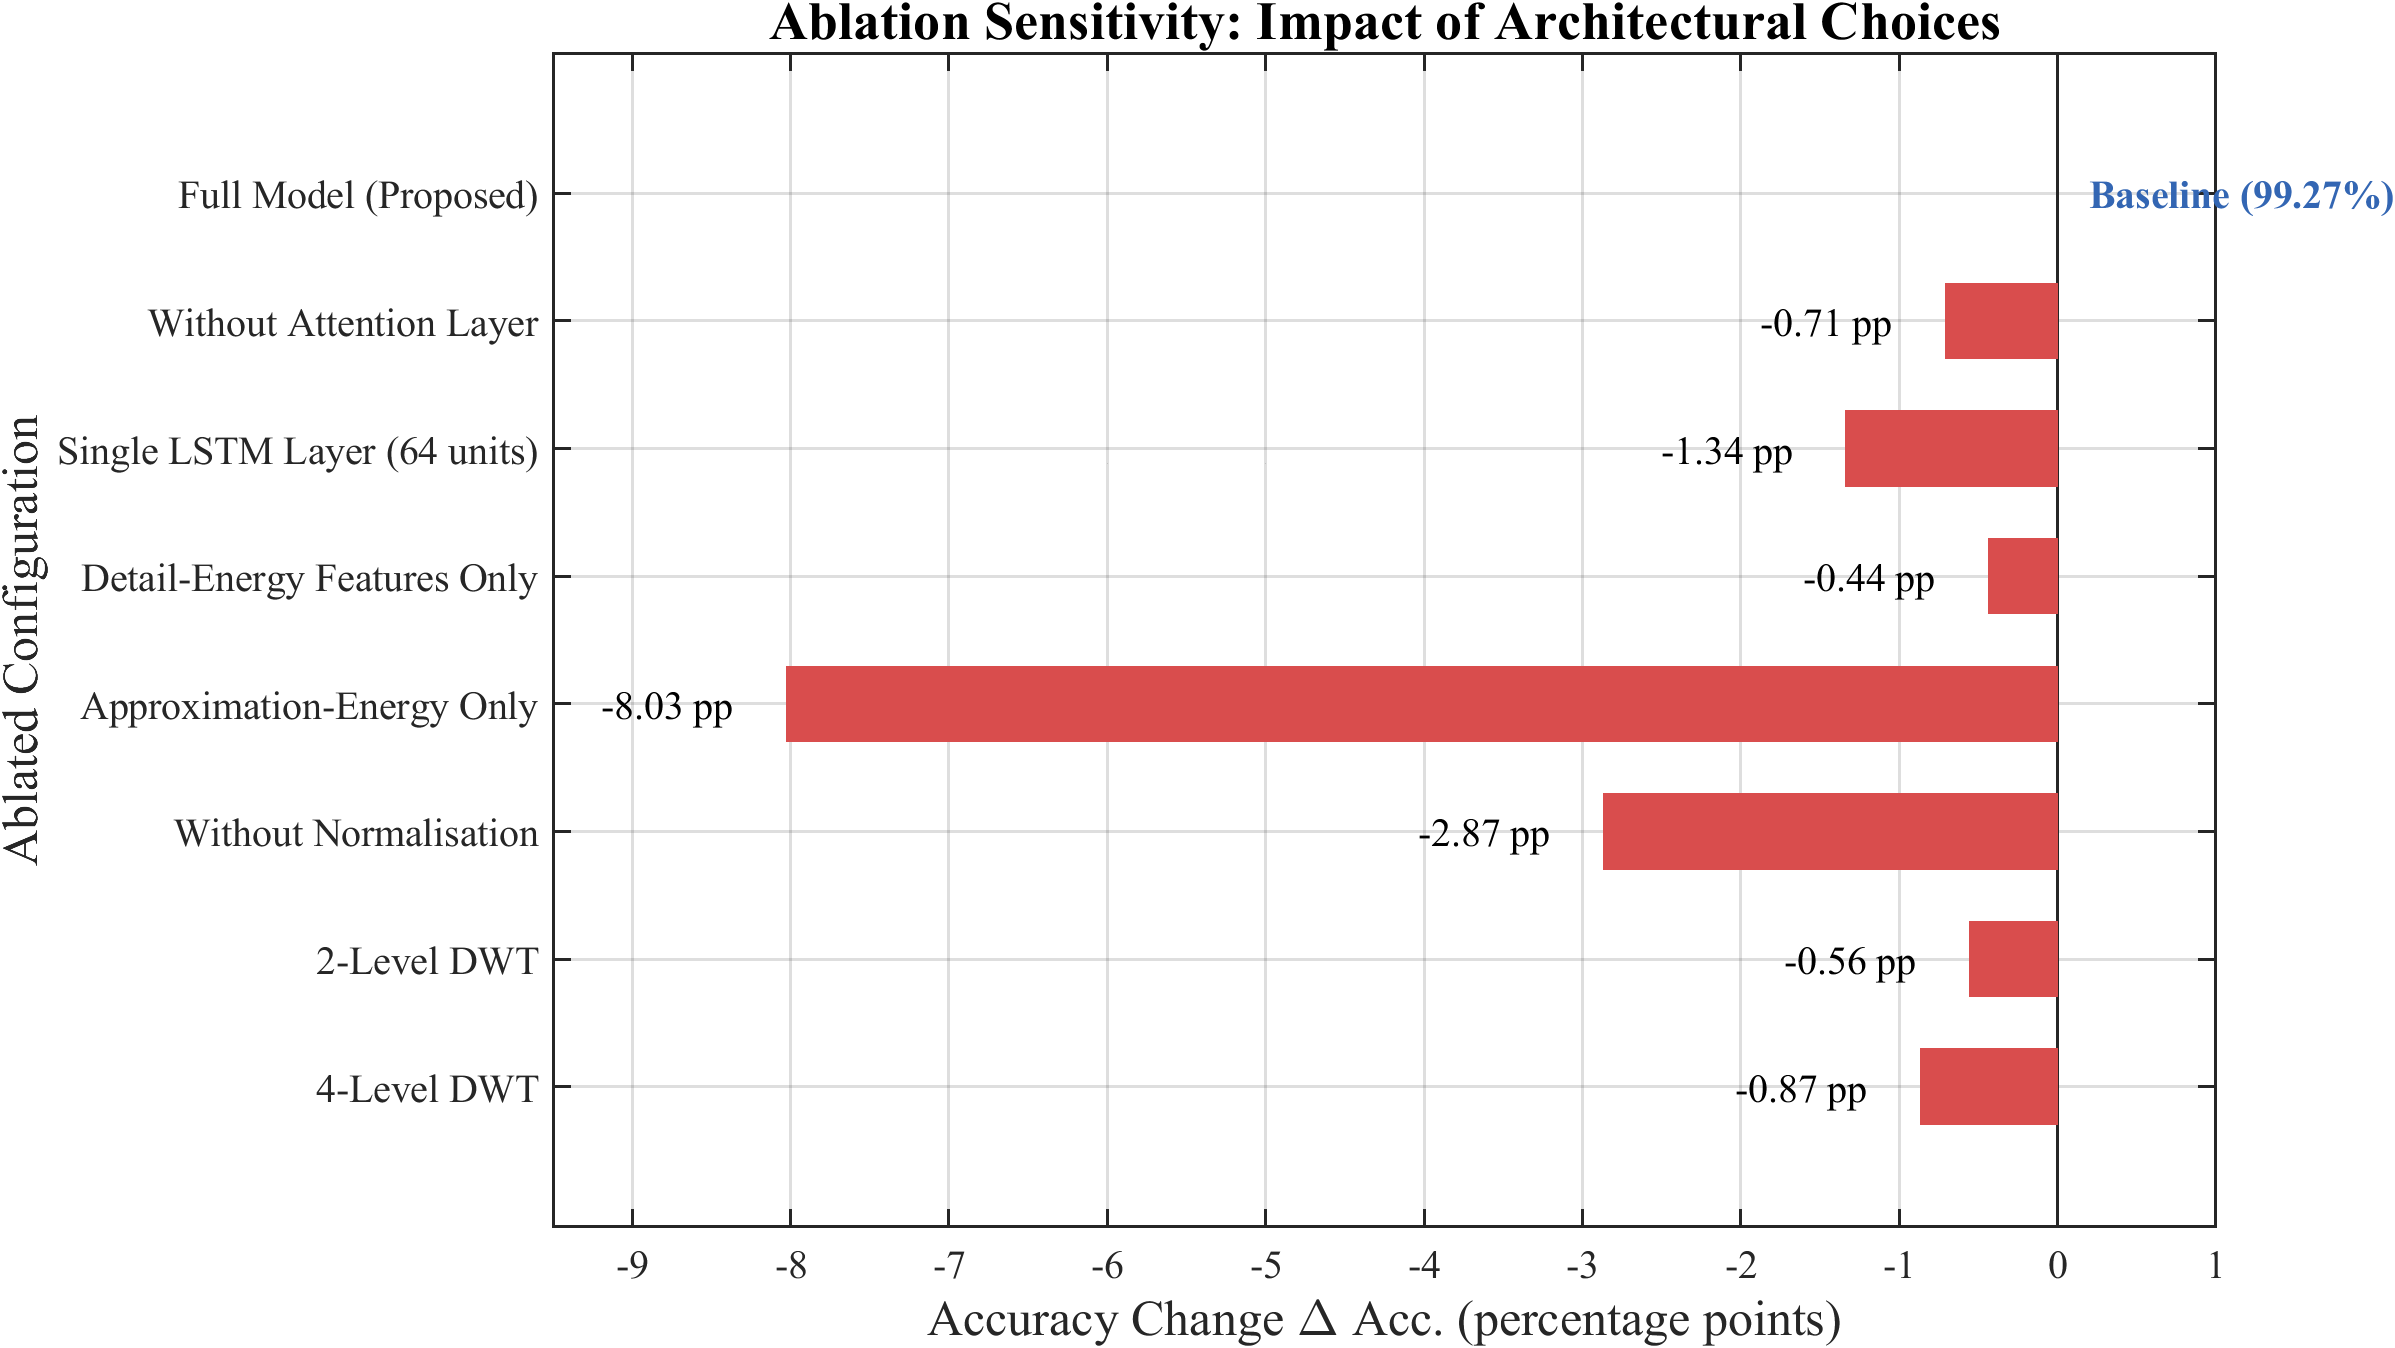
\includegraphics[width=0.75\textwidth]{figures/ablation_sensitivity_tornado.png}
\caption{Ablation sensitivity of classification accuracy to individual design choices.}
\label{fig:ablation_tornado}
\end{figure}

\begin{figure}[htpb]
\centering

\includegraphics[width=0.75\textwidth]{figures/academic_plots/04_ROC_and_PR_Curves.png}
\caption{ROC curve for internal-fault detection with the selected confidence-threshold operating point.}
\label{fig:roc_curve}
\end{figure}

\begin{figure}[htpb]
\centering

\includegraphics[width=0.75\textwidth]{figures/academic_plots/09_Confidence_Distribution.png}
\caption{Learned temporal-attention weight distribution across the input window for each event type.}
\label{fig:attention_heatmap}
\end{figure}
